\documentclass{article}
\usepackage{verbatim,
            mathtools,
            amsmath,
            graphicx}

\title{This is LaTex on VS Code}
\author{Tariq Erwa}
\date{2021-2-24}

\begin{document}
 %this is a single line comment
   \begin{comment}
      This
      is
      a
      multi
      line
      comment
   \end{comment}
   \pagenumbering{gobble}
   \maketitle
   \newpage
   \pagenumbering{arabic}
   \section*{Objective}
       Lab report stuff...
   %how to use math expressions
   \section*{Theory}
   Newotons Second Law was
   \begin{equation}\label{a}
      F=ma
   \end{equation}

   it can also be written as

   $$
   F_{net} = m \cdot \frac{d^2 y}{d x^2} 
   $$
   Or as

   \[
   \sum F = ma
   \]

   for an oscilating object the restoring force is : $F = -kx$ \\ 
   so the net force 
   \begin{align*}
      F &= ma\\
      &= -kx 
   \end{align*}
   
   a possible solution for this differential equation is

   $$
   x =A \sin (t)
   $$
   \section*{Other Examples}
   \begin{itemize}
      \item Limits:
         $$
         \lim_{x \to \infty} e^{-x} = 0
         $$
      \item Roots:
         $$
         \sqrt[3]{x}
         $$
      \item Table:
         \begin{table}[ht]
            \centering
            \begin{tabular}{|c|c|c|}
               \hline
               4 & 3 & 9 \\
               \hline
               8 & 4 & 3 \\
               \hline
               7 & 9 & 0 \\
               \hline
            \end{tabular}
            \caption{shows the readings of randomness}

         \end{table}
            
         
         hbuhb 
      \newpage
      \item : Figure
         \begin{figure}
            \caption{shows lazyness}
            %didn't include it because am lazy
            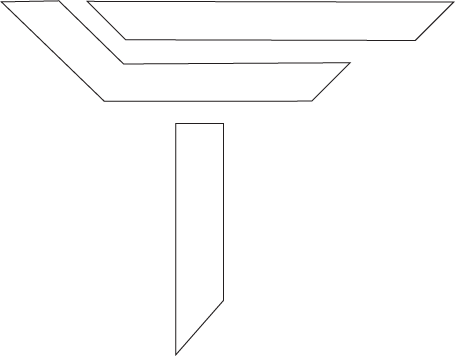
\includegraphics{Untitled-1.png}
         \end{figure}
   \end{itemize}
\end{document}
